\chapter{R3 hardvér}
\label{kap:2}
Nasledujúca kapitola je venovaná vyhotoveniu zariadenie z pohľadu hardwaru. Hovorí o častiach, z ktorých sa zariadenie skladá, o ich parametroch, funkciách a vlastnostiach. Taktiež porovnáva poslednú verziu vyhotovenia – verzia R3, so staršími verziami zariadenia, vysvetľuje, prečo sme sa pre dané zmeny rozhodli a ako vplývajú na celkové fungovanie zariadenia. Najskôr sa vyjadruje k mechanickej časti a následne, ku použitým komponentom ako je servo motor alebo snímače. 

\section{Schéma zapojenia}
\label{kap:2.1}

Schéma zapojenia nášho zariadenia prešla od poslednej verzie niekoľkými zmenami. Celkovo by sa dala rozdeliť na 2 oddelené schémy, ktoré sú vzájomne prepojené pomocou FFC (flat flexible cable) káblu. Oddelenie schém je potrebné z dôvodu, že senzory na snímanie polohy guličky v trubičke a pootočenia ramena musia byť umiestnené na trubičke. Z toho vyplýva že schéma celého našeho zariadenia musí byť oddelená aby mohli byť vytvorené 2 PCB dosky, ktorú v celku tvoria jednu schému. Prvou je časť zariadenia nachádzajúca sa na hlavnej PCB doske, ktorú priamo zapájame do Arduina. Obsahuje kondenzátory a diódu potrebné pre správne fungovanie pripojených komponentov, ďalej kontakty na pripojenie Serva a FFC kábla. Najväčšou zmenou je však implementácia lineárneho regulátora napätia (LDO) \ref{kap:2.2.4}, ktorý je potrebný pre úpravu napätia do rozsahu vhodnom pre fungovanie súčiastok.
\begin{figure}[!h]
	\centering
	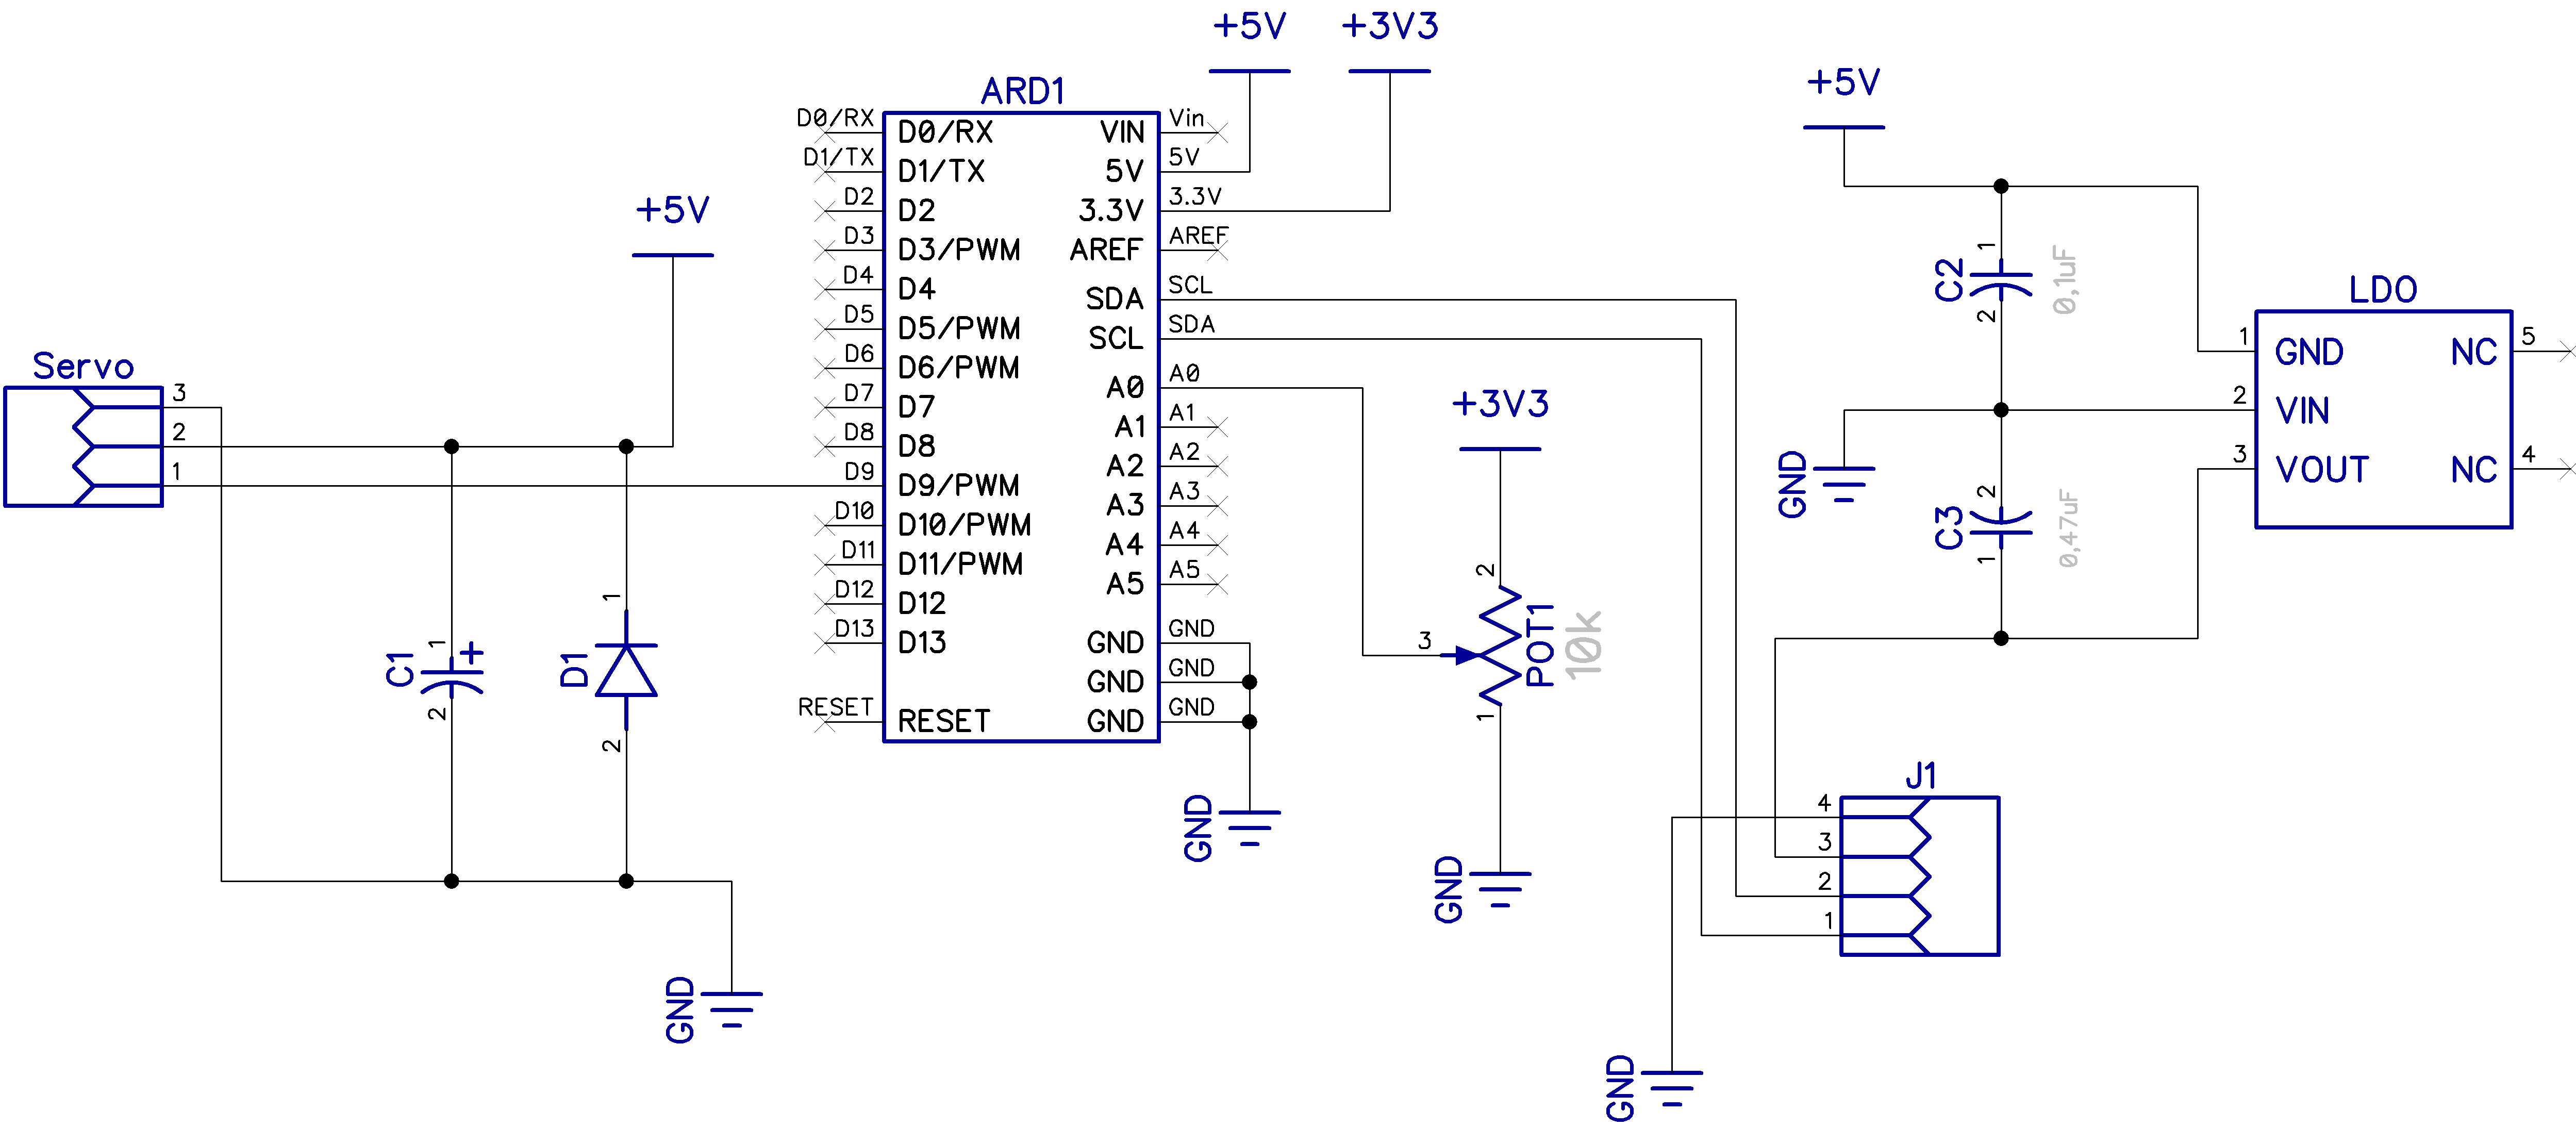
\includegraphics[width=150mm]{obr/BoBshield.png}
	\caption{Schéma hlavnej PCB dosky}\label{OBRAZOK 2.1.1} 
\end{figure} 

Druhá časť schémy je nami navrhnutá breakout doska, nachádzajúca sa v koncovej polohe trubičky a obsahuje hore spomenuté snímače polohy guličky a pootočenia ramena. Konkrétne ide o ToF (time of flight) snímač VL6180X a gyroskop MPU 6050. Taktiež sa v nej nachádzajú kondenzátory a rezistory a kontakt na pripojenie FFC kábla. V porovnaní s predošlou verziou kde bola táto PCB doska riešená už hotovým breakoutom od výrobcu sa nám podarilo zmenšiť jej rozmery a to aj napriek implementácii ďalšieho snímača a konektoru na FFC kábel. 

\begin{figure}[!h]
	\centering
	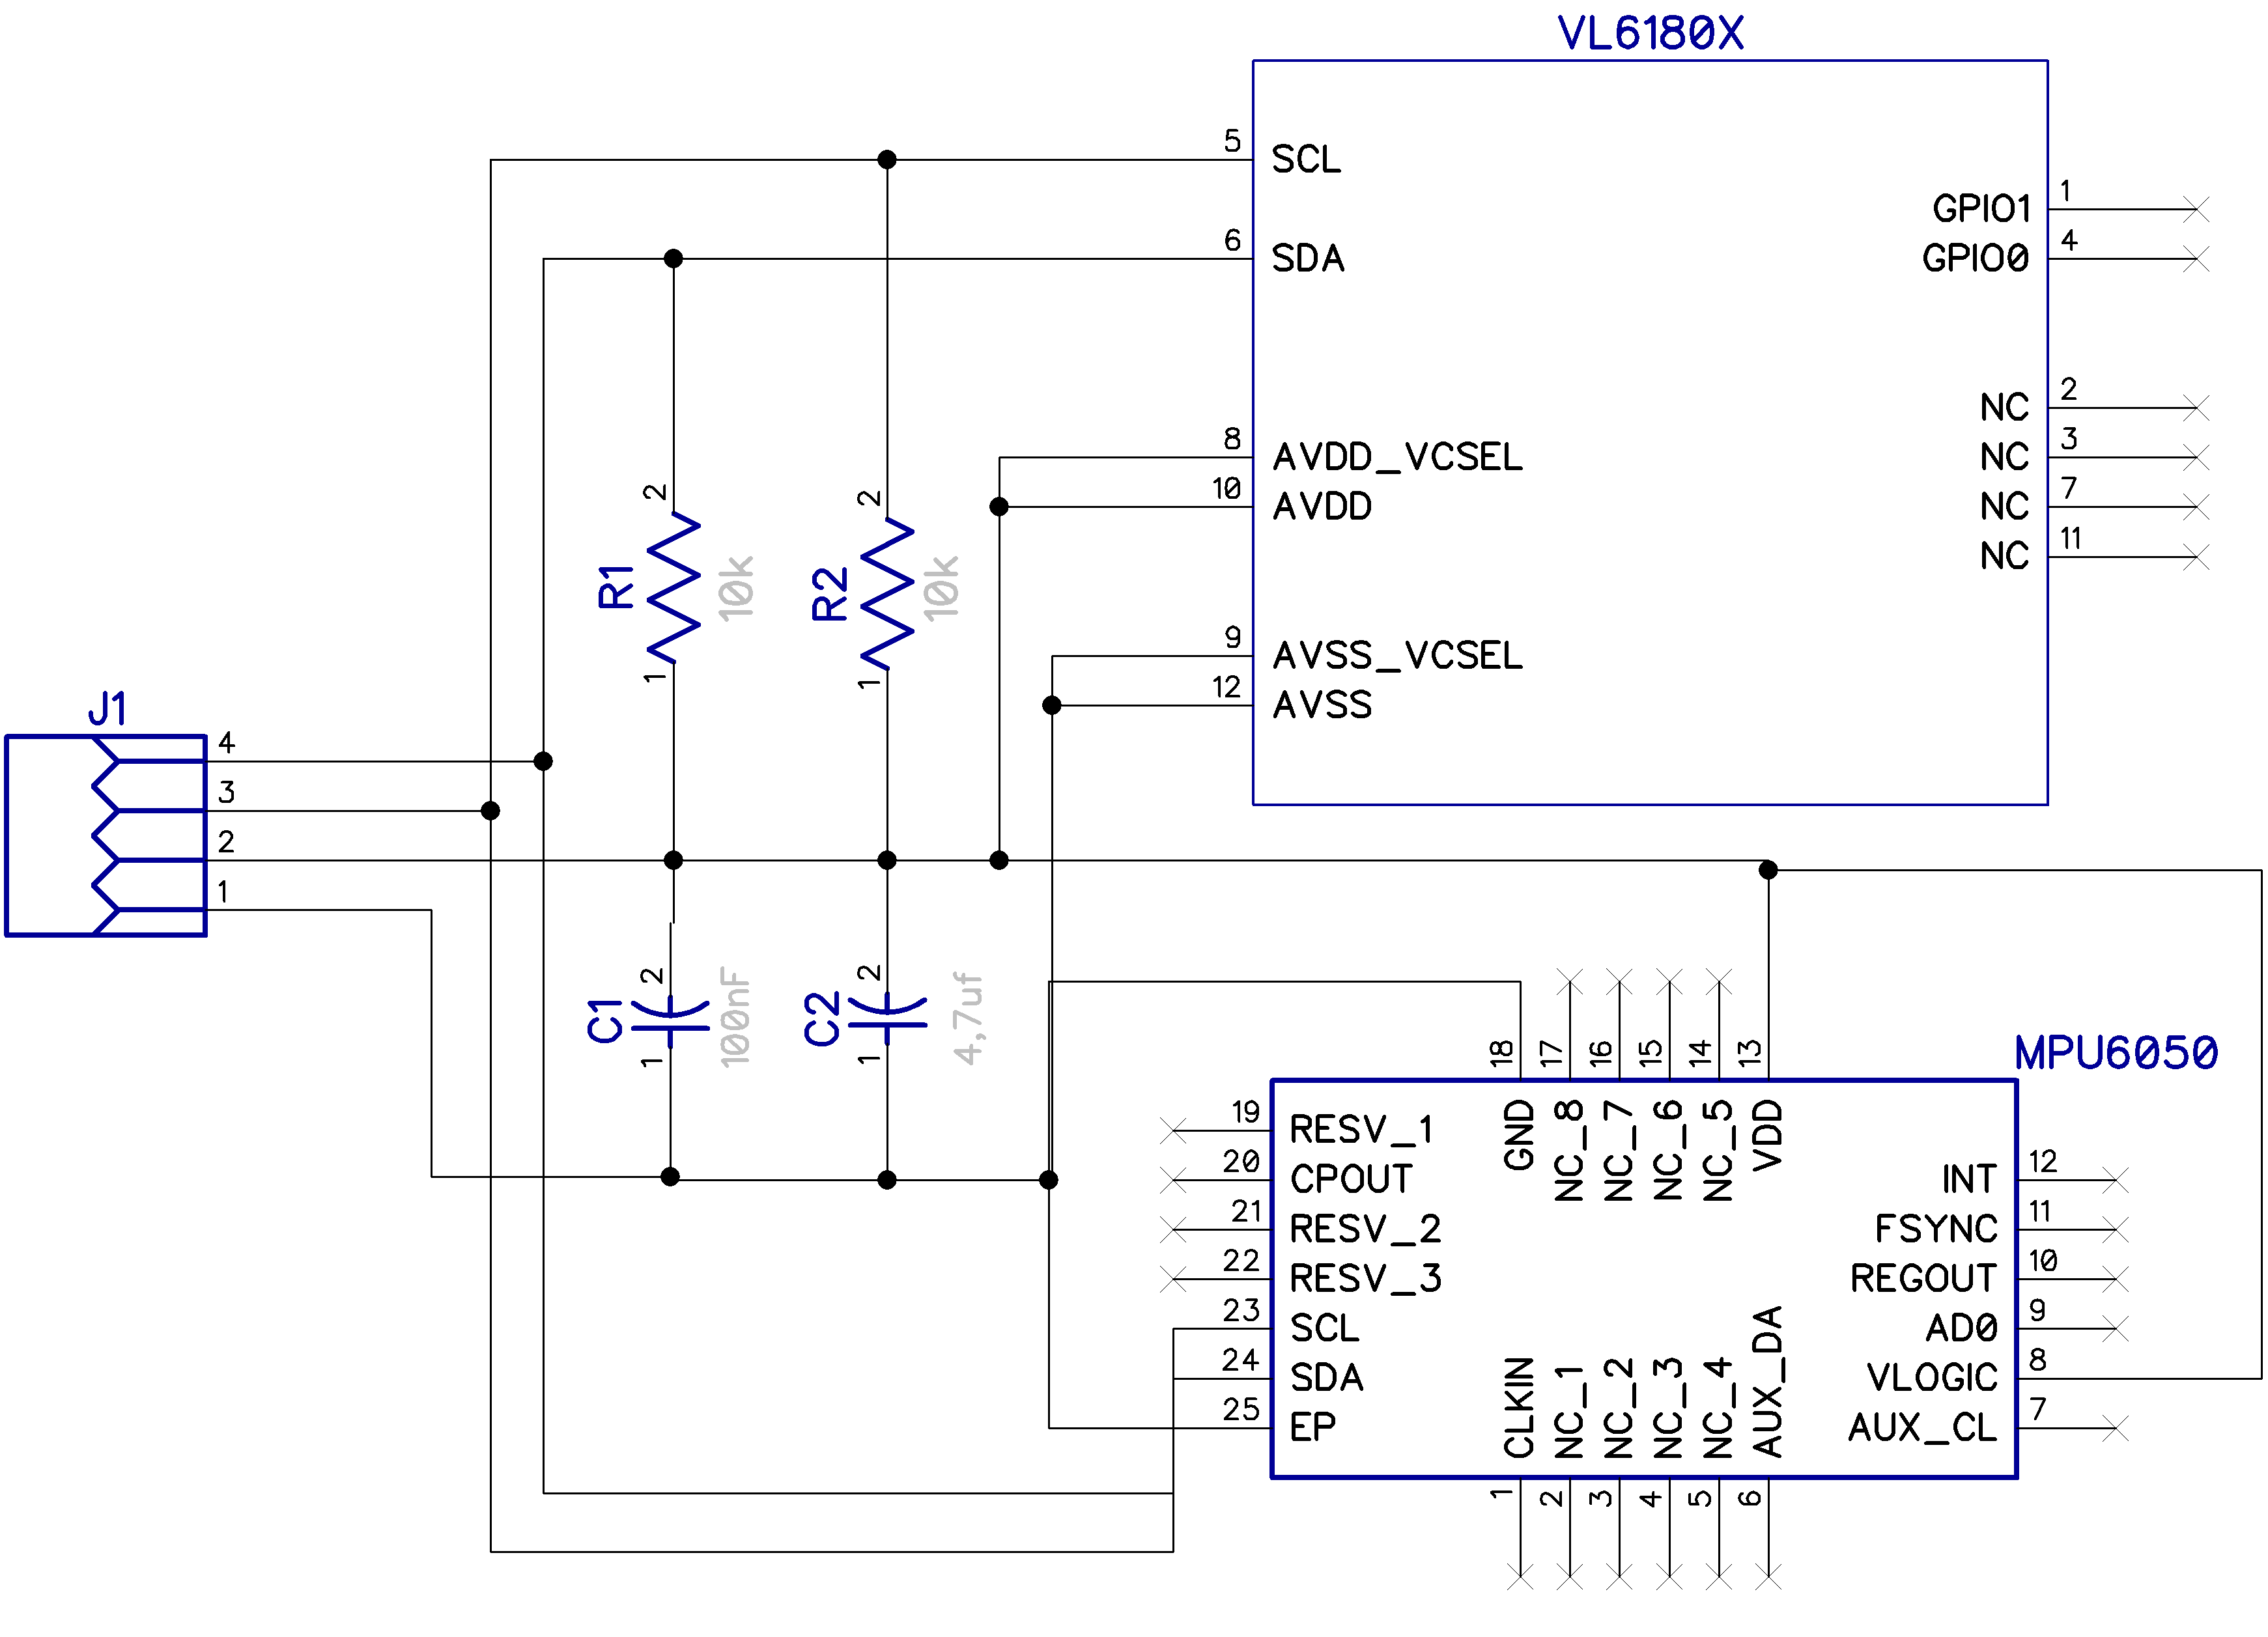
\includegraphics[width=100mm]{obr/senzors.png}
	\caption{Schéma PCB dosky so snímačmi}\label{OBRAZOK 2.1.2} 
\end{figure} 

Obe schémy boli navrhnuté vo voľne dostupnom software DIPTrace. 
 
% Obrázky schém + opis 
% Obrázky PCB dosiek + opis
 
 
\section{Komponenty}
\label{kap:2.2}

Pre riadenie a regulovanie akéhokoľvek systému je potrebné mať vstup do systému, ktorý v zariadeniach získavame pomocou snímačov, a taktiež potrebujeme aby výstup z riadiaceho systému mohol ovplyvňovať riadený systém. Zásah do systému na základe výstupu z riadiaceho systému majú na starosti aktuátory. 

V našom zariadení sa o jednotlivé funkcie starajú nasledujúce komponenty:
\begin{itemize}
    \item snímače – Tof snímač vzdialenosti, Gyroskop
	\item aktuátory – Servo motor 
\end{itemize}


\subsection{Servo}
\label{kap:2.2.1}

\subsection{ToF snímač - VL6180X}
\label{kap:2.2.2}

Pri snímači vzdialenosti sme sa rozhodli ostať pri pôvodnej voľbe typu a modelu, ktorým je VL6180X.
Ide o ToF snímač, ktorý meria vzdialenosť na základe vysielania, odrazu a následného prijímania svetelného lúča. Princíp fungovanie(obr. \ref{OBRAZOK 2.2.2}) je založený na meraní času, za ktorý svetelný lúč vyslaný zo snímača doletí k telesu, ktorého pozíciu meriame, odrazí sa od neho a vráti sa späť. Na základe rovnice (rov. \refeq{rovnica.2.1}), kde  \(c\) - predstavuje rýchlosť svetla, \(\Delta T\) – čas, ktorý trvá lúču odraz a návrat k snímaču, samotný snímač vypočíta vzdialenosť - \(x\) , v ktorej sa nachádza teleso od snímača. Komunikácia s arduinom prebieha prostredníctvom I2C protokolu. Rozsah napájacieho napätie je 2,6V – 3,0V. 
\begin{align}
	\label{rovnica.2.1}
	2x = c*\Delta T
\end{align}
\begin{figure}[!h]
	\centering
	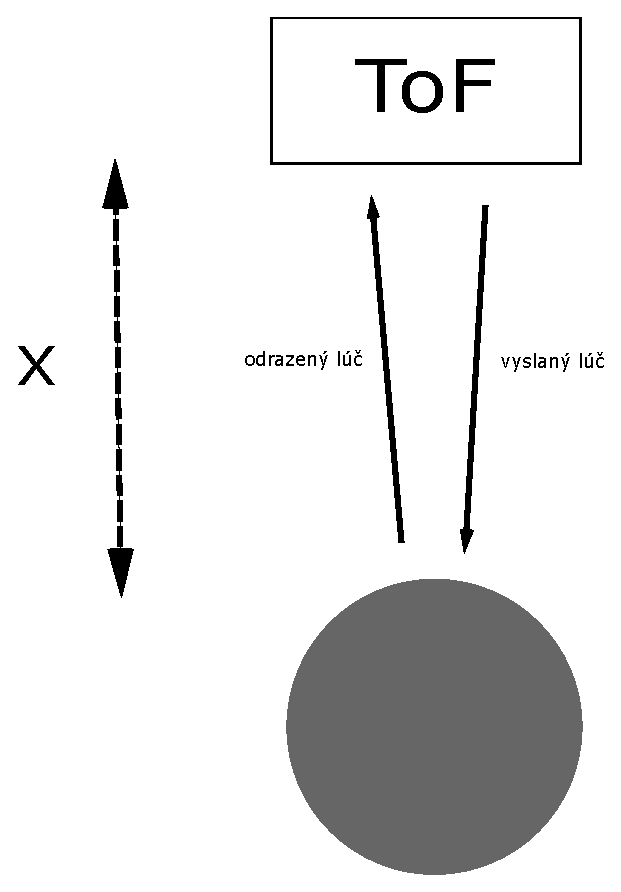
\includegraphics[width=60mm]{obr/ToF.eps}
	\caption{Princíp fungovania ToF senzora}\label{OBRAZOK 2.2.2} 
\end{figure} 

Hoci sme zvažovali aj iné typy snímačov vzdialenosti ako napríklad ultrazvukové alebo IR (infračervené) snímače, prišli sme k záveru, že najvhodnejším typom snímača bude práve ToF vďaka jeho malým rozmerom. Z možností ToF snímačov ponúkaných na trhu je pre naše zadanie VL6180X momentálne ideálnou možnosťou z dôvodu:
\begin{itemize}
	\item merateľného rozsahu - 100 mm
	\item presnosti merania - na 1 mm 
	\item malým rozmerom – 4.8 x 2.8 x 1.0 mm
\end{itemize}

Merateľný rozsah snímača je pre nás úplne postačujúci, keďže gulička sa pohybuje v trubičke práve o dĺžke 100 mm, s tým že v koncových bodoch sa nachádzajú ešte uzavretia trubičky, takže rozsah pohybu guličky je približne 90 mm, čo nám dáva ešte určitú rezervu. Taktiež presnosť meranie na 1 mm je pre riadenie systému dostatočná. Rozmery sú pre nás dôležité z hľadiska potreby umiestnenia snímača do jednej z koncových polôh trubičky aby sme mohli merať pozíciu guličky. Taktiež príliš veľké rozmery ako napríklad pri ultrazvukovom snímači by nepriaznivo vplývali na pohyb trubičky okolo osi otáčania, nehovoriac o estetickosti zariadenia. Vďaka minimálnym rozmerom snímača sa nám oproti pôvodnej verzii podarilo zmenšiť diel upevnenia snímača na trubičke, čím sme zlepšili aj estetickú zložku zariadenia.
Úlohou snímača je snímať polohu guličky v trubičke a dáta posielať mikropočítaču. Poskytuje nám aktuálnu hodnotu vzdialenosti, ktorá sa porovnáva s požadovanou na základe čoho regulátor vypočíta hodnotu akčného zásahu do systému.


\subsection{Gyroskop - MPU 6050}
\label{kap:2.2.3}

Snímač MPU 6050 je oproti pôvodným verziám zariadenia úplnou novinkou. Ide o 6 osový snímač pohybu – 3 osový gyroskop a 3 osový akcelerometer zostavený v malom balený o rozmeroch 4 x 4 x 0,9 mm. Jeho využitie je veľmi široké a stretnúť sa s ním môžeme pri smartfónoch alebo tabletoch. Poskytuje možnosti využívané pri aplikáciách ako navigácia, rozšírená realita, monitorovanie zdravia a pohybu a mnoho ďalších. Snímač užívateľovi poskytuje možnosť nastavenia meraného rozsahu v závislosti od aplikácie, pre ktorú bude využitý, teda pre sledovanie jednak rýchlych aj pomalých pohybov. Pri gyroskope si užívateľ môže vybrať z nasledujúcich rozsahov - ±250, ±500, ±1000 a ±2000\textdegree /s. U akcelerometra ide o rozsahy ±2g, ±4g, ±8g a ±16g.  Komunikácia s arduinom prebieha rovnako ako pri ToF snímači prostredníctvom I2C protokolu a rozsah napájacieho napätia 2,375V – 3,46 V.  

Jeho úlohou je merať uhol natočenia trubičky, na základe čoho vieme nastaviť trubičku do vodorovnej polohy.  



\subsection{Lineárny regulátor napätia - LDO}
\label{kap:2.2.4}

Z dôvodu tvorby vlastného braekoutu, na ktorom sú umiestnené oba naše snímače bolo potrebné nájsť vhodné napájacie napätie aby vyhovovalo obom snímačom a spadalo do ich rozsahov napätí. Pre snímač VL6180X je vstupné napätia v rozmedzí 2,6 V - 3,0 V a pri MPU6050 ide o rozsah 2,375 – 3,46 V. Arduino nám ponúka len 2 úrovne napájania a to 3,3 V a 5 V. Ak by sme využívali len snímač MPU6050 mohli by sme priamo využiť napájanie 3,3 V, ktoré spadá do jeho pracovného rozsahu, no pre snímač polohy je táto možnosť nevyhovujúca. Preto je potrebné upraviť ponúkané úrovne napätia z arduino dosky do rozsahu 2,6 - 3,0 V, vyhovujúcemu obom snímačom. O zmenu napätia sa stará lineárny regulátor napätia – STM732M28R od firmy STMicroelectronics , ktorý vstupné napätie v rozsahu 2,5 – 28 V prevádza na úroveň 2,8 V. Táto hladina je vyhovujúca pre oba snímače.   


\section{Teleso}
\label{kap:2.3}

Dôležitou časťou celého systému je práve gulička, pohybujúca sa v trubičke, ktorej polohu sledujeme a riadime. Na náš systém vplýva ako jej hmotnosť a tvar tak aj kvalita a farba jej povrchu. Keďže na meranie polohy guličky používame ToF snímač, ktorý meria vzdialenosť na základe času, za ktorý sa svetelný lúč vyslaný zo senzora odrazí od telesa a vráti naspäť, na kvalitu merania vplývajú aj tieto parametre. Hoci výrobca v datasheetoch {ref datasheet}uvádza nezávislosť merania snímača od farby alebo kvality povrchu telesa, po našich meraniach sme mohli sledovať odlišnosti v presnosti pre rôzne typy guľôčok. Tento fakt môže byť ovplyvnený práve tvarom meraného telesa, ktorý v našom prípade nie je ideálny, no pre potreby nášho zadania nevyhnutný. Svetelný lúč nedopadá na kolmý povrch, preto nemusí byť odrazený práve pod takým uhlom aby ho dokázal snímač adekvátne zachytiť a zanalyzovať. Na základe tohto faktu sme predpokladali, že by ideálnym riešením bolo teleso s povrchom, ktorý čo najviac rozptýli dopadajúci lúč aby pravdepodobnosť, že sa lúč od neho odrazí k snímaču bola čo najvyššia, čím by sa zlepšila kvalita merania. Ďalšou požiadavkou pri hľadaní ideálneho telesa bola dostatočná hmotnosť guličky aby bol systém dynamický a dokázal aktívne reagovať na zmeny pootočenia ramena. Aby sa gulička mohla voľne pohybovať v trubičke, nič jej nebránilo a tak nevplývalo na systém je potrebné aby bol jej tvar čo najviac podobný tvaru ideálnej gule. Poslednou požiadavkou bola jeho jednoduchá dostupnosť. Keďže sa jedná o open source projekt, je potrebné aby sa každý, kto by mal záujem o zostrojenie nášho zariadenia vedel ku danej guličke bez väčších problémov dostať.

Z možností dostupných na trhu sme sa rozhodli otestovať náš snímač  pre viacero typov materiálov: 
 drevo, silikón, POM - polyoxymetylén, NBR - butadien-akrilonitrilový kaučuk (syntetická guma), NR - prírodná guma, oceľa PP - polypropylén.


Pri meraní sme postupovali nasledovne. Guličku sme nastavili do krajnej polohy v trubičke (vzdialenosť 90 mm), následne sme pomocou ToF snímača zmerali 100 hodnôt jej aktuálnej polohy. Hodnoty sme vložili do tabuľky a pomocou vzorca sme vypočítali smerodajnú odchýlku pre dané meranie. Tento postup sme zopakovali pre všetky materiály. V tabuľke \ref{TABULKA_2_1} môžeme vidieť porovnanie smerodajných odchýlok pre jednotlivé materiály. Na základe merania, ktoré sme vykonali, môžeme tvrdiť, že náš snímač dosahuje najväčšiu presnosť pri materiály PP – polypropylén a najväčšie odchýlky pri NBR – syntetická guma. 


\begin{table}[ht]
	\centering
    \begin{tabular}{|l|l|l|l|l|l|l|l|}
    	\hline
    	\textbf{Materiál}            & silikón & POM    & drevo  & NBR                            & NR     & oceľ & PP                             \\ \hline
    	\textbf{smerodajná odchýlka} & 1,27    & 1,2891 & 1,3644 & \cellcolor[HTML]{FFCCC9}1,6271 & 1,3322 & 1,5  & \cellcolor[HTML]{9AFF99}1,2595 \\ \hline
    \end{tabular}
	
    \caption{Smerodajné odchýlky pre dané materiály}
    \label{TABULKA_2_1}
\end{table}
Ako bolo vyššie spomenuté, dynamika systému má veľký vplyv na jeho riadenie. Z toho dôvodu je pri výbere guličky dôležitá práve rýchlosť akou sa gulička v systéme pohybuje. Ak je gulička príliš rýchla  , riadiaci systém má menej času reagovať na zmenu jej polohy, ktorá sa hlavne pri výraznej zmene referenčnej hodnoty výrazne mení. Keďže dĺžka trubičky je pomerne malá (100 mm), ak riadiaci systém nedokáže včas zareagovať  na zmenu jej polohy bude dochádzať k nárazom guličky do krajných polôh trubičky, čo je pri riadení nežiaduci jav. Z toho dôvodu sa snažíme voliť guličku, ktorej rýchlosť je adekvátna pre našu aplikáciu. Rýchlosť guličky je závislá jednak od jej hmotnosti, materiálu, kvality povrchu a rozmerov.
Pri meraní sme zaznamenávali polohu guličky a čas, v ktorom sa v danej polohe nachádzala. Pohyb guličky bol z jednej krajnej polohy trubičky do druhej krajnej polohy pri naklonení trubičky o čo najmenší uhol. Následne sme namerané hodnoty vykreslili do grafu v programe MATLAB a pomocou analýzy grafu sme našli čas, za ktorý gulička prešla danú vzdialenosť trubičky. Hodnoty sme zapísali do tabuľky a vypočítali rýchlosť jednotlivých guličiek.

\begin{table}[ht]
	\centering
	\begin{tabular}{|l|l|l|l|l|l|l|l|}
		\hline
		\textbf{Materiál}           & silikón & POM    & drevo  & NBR                            & NR     & oceľ                           & PP                             \\ \hline
		\textbf{rýchlosť {[}m/s{]}} & 0,0862  & 0,1035 & 0,1178 & \cellcolor[HTML]{9AFF99}0,0766 & 0,1128 & \cellcolor[HTML]{FFCCC9}0,1214 & \cellcolor[HTML]{FFFFFF}0,0895 \\ \hline
	\end{tabular}
    \caption{Rýchlosti guličiek pre dané materiály}
    \label{TABULKA_2_2}
\end{table}

V tabuľke \ref{TABULKA_2_2} môžeme vidieť porovnanie rýchlosti jednotlivých guličiek pri pohybe mierne naklonenou trubičkou. Najpomalšie sa pohybujúcou je gulička z NBR, ktorá oproti guličke z ocele, použitej v pôvodných verziách zariadenia dosahuje takmer polovičné priemerné rýchlosti.  
Na základe vykonaných meraní sme sa rozhodli zvoliť si za teleso v systéme guličku vyrobenú z polypropylénu (PP). Snímač dosahuje pri danej guličke najpresnejšie merania, takže meraná poloha guličky sa najviac približuje jej skutočnej polohe. Presné meranie je pri riadení systému kľúčové, no treba uvažovať aj dynamiku guličky. Z nameraných rýchlostí guličiek by pre nás bola najvhodnejšou voľbou gulička z NBR, no jej presnosti merania sú výrazne horšie v porovnaní s guličkou PP. Tá ale dosahuje tiež prijateľné rýchlosti pre náš systém, preto je momentálne optimálnou voľbou.
Ak porovnáme guličku z ocele, ktorá je telesom použitým v pôvodnej verzii

\section{Prevod rotačného pohybu - servo, trubička}  \textdegree
\label{kap:2.4}

Aktuátorom v našom zariadení je servo motor, no aby mohol vytvárať akčný zásah (pootočenie trubičky) do systému, ktorým je naša trubičke s guličkou, musí prísť ku prenosu rotačnému pohybu.
 
V pôvodnej verzii zariadenia bol tento prevod riešený priamym upevnením trubičky na Servo motor, čo znamená, že otočenie trubičky sa rovnalo otočeniu serva o príslušný uhol z rozsahu ±30\textdegree, ktorý bol stanovený. Najmenší možný uhol pootočenia trubičky sa teda rovnal presnosti serva - 1\textdegree. To je vzhľadom na dĺžku trubičky pomerne veľký uhol a pri riadení systému tak aktuátor obmedzuje výstup z riadiaceho systému a akčný zásah do systému na pomerne hrubé a nie tak presné hodnoty. 

Našim riešením tohto problému je použitie jednoduchého prevodu, cez ktorý budeme prenášať rotačný pohyb serva na trubičky. Prevod sa skladá z 2 koliesok rozdielnych priemerov, pričom jedno je upevnené na servo motor a k druhému je pripevnená trubička. Prenos pohybu z jedného kolieska na druhé je riešené pomocou ozubeného remeňa GT2 o šírke 6 mm, bežne používanom pri krokových motoroch. Výhodou nášho riešenia je využitie takmer celého rozsahu pohybu nášho servo motora. Kým pri pôvodnom zariadení išlo o využitie rozsahu ±30\textdegree z možných ±90\textdegree,  v danom riešení využívame rozsah ±75\textdegree.

Prevodový pomer - $p$ a následne aj rozmery koliesok ($d1$ - vstupný priemer, $d2$ - výstupný priemer) sme vypočítali na základe vzorcov (\ref{rovnica.2.4.1}) pre výpočet prevodov, kde najprv zistíme prevodový pomer na základe vstupného a výstupného rozsahu otočenia. Vzorce sa dajú jednoducho odvodiť na základe dĺžky posunutia remeňa - x, ktorá je na oboch kolieskach vždy rovnaká. Ide o dĺžku kružnicového oblúka, o priemere daného kolieska, ktorého uhol je rovný uhlu otočenia (obr.\ref{OBRAZOK 2.4.1}). Tento uhol môžeme pri výpočtoch nahradiť rozsahom otáčania jednotlivých koliesok.  Za výstupný rozsah sme si zvolili ±15\textdegree, pre dĺžku trubičky je tento uhol postačujúci keďže referenčná hodnota sa pohybuje od 0 po 100 mm a gulička sa pohybuje v trubičke dostatočne veľkou rýchlosťou bez väčšieho odporu, nemusí dochádzať k tak výrazným zásahom aktuátora ako je naklonenie o celých 30\textdegree, či už kladným alebo záporným smerom.  Reakcia systému je aj pri nami zvolenom rozsahu dostatočne rýchla. Pre vstupný rozsah sme si zadali ±75\textdegree aby sme disponovali určitou rezervou voči maximálnemu rozsahu otočenia.



\begin{align}
	\label{rovnica.2.4.1}
	p &= \frac{d1}{d2} \\
	x_1&=\frac{\pi*d_1*\alpha_1}{360} \\
	x_2&=\frac{\pi*d_2*\alpha_2}{360}
\end{align}

\begin{figure}[!h]
	\centering
	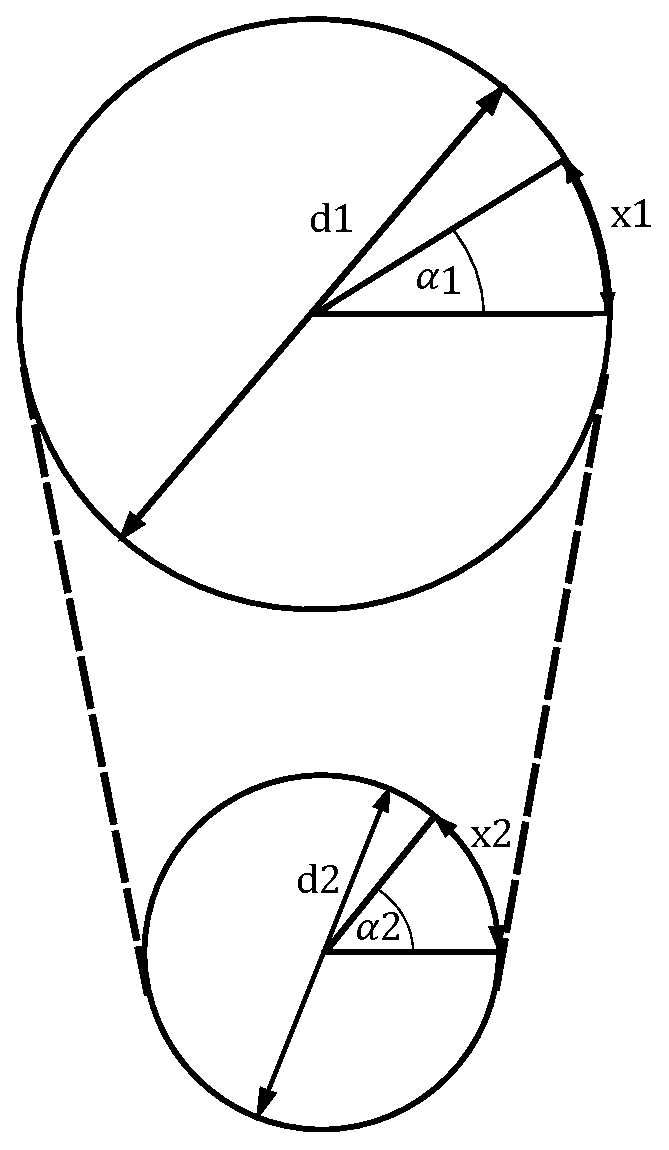
\includegraphics[width=50mm]{obr/prevod.eps}
	\caption{Posunutie remeňa pri rotácii kolieska}\label{OBRAZOK 2.4.1} 
\end{figure} 

\begin{align}
	\label{rovnica.2.4.2}
		x_1 &= x_2 \\
	p &=\frac{d_1}{d_2}=\frac{\alpha_1}{\alpha_2} \\
	p &=\frac{30\degree}{150\degree}=0.2
\end{align}
Na základe prevodového pomeru vieme povedať, že na 1\textdegree otočenia serva prislúcha 0,2\textdegree otočenia trubičky. Týmto prevodom sme teda 5 násobne zväčšili počet hodnôt , ktoré môže aktuátor nadobudnúť a tým zvýšili presnosť akčného zásahu do systému. 
Ak poznáme prevodový pomer rozmery koliesok získame voľbou priemeru jedného z nich a následným výpočtom priemeru druhého kolieska na základe vzorca \ref{rovnica.2.4.1}. Za priemer kolieska pripojeného k servo motoru sme si zvolili $d1 = 10 mm$. Je to dostatočná veľkosť pre uchytenie kolieska a prevod pohybu pomocou remeňa, no zároveň šetríme miesto aby sme zachovali minimálne rozmery pôvodnej verzie zariadenia. Z toho vyplýva, že priemer druhého kolieska bude $d2 = 50 mm$.  





\section{3D prvky}
\label{kap:2.5}

Z dôvodu zmeny použitých komponentov, došlo aj k potrebe aktualizácie a úprave 3D prvkov použitých v našom zariadení. 